\documentclass{vkr}
\usepackage[english, russian]{babel} % переносы
\usepackage{graphicx} % для вставки картинок
\graphicspath{{images/}} % путь к изображениям
\usepackage[hidelinks]{hyperref}
\usepackage{float} % определяет метод H для рисунка с переносом на следующую страницу, ели не помещается
\usepackage{pdflscape}
\addto{\captionsrussian}{\renewcommand{\refname}{СПИСОК ИСПОЛЬЗОВАННЫХ ИСТОЧНИКОВ}}
\usepackage{xltabular} % для вставки таблиц
\usepackage{makecell}
\renewcommand\theadfont{} % шрифт в /thead
\usepackage{array} % для определения новых типов столбцов таблиц
\newcolumntype{T}{>{\centering\arraybackslash}X} % новый тип столбца T - автоматическая ширина столбца с выравниванием по центру
\newcolumntype{R}{>{\raggedleft\arraybackslash}X} % новый тип столбца R - автоматическая ширина столбца с выравниванием по правому краю
\newcolumntype{C}[1]{>{\centering\let\newline\\\arraybackslash\hspace{0pt}}m{#1}} % новый тип столбца C - фиксированная ширина столбца с выравниванием по центру
\newcolumntype{r}[1]{>{\raggedleft\arraybackslash}p{#1}} % новый тип столбца r - фиксированная ширина столбца с выравниванием по правому краю
\newcommand{\centrow}{\centering\arraybackslash} % командой \centrow можно центрировать одну ячейку (заголовок) в столбце типа X или p, оставив в оcтальных ячейках другой тип выравнивания
\newcommand{\finishhead}{\endhead\hline\endlastfoot}
\newcommand{\continuecaption}[1]{\captionsetup{labelformat=empty} \caption[]{#1}\\ \hline }
\usepackage{etoolbox}
\AtBeginEnvironment{xltabular}{\refstepcounter{tablecnt}} % подсчет таблиц xltabular, обычные таблицы подсчитываются в классе

\usepackage[tableposition=top]{caption} % подпись таблицы вверху
\captionsetup{strut=off}
\setlength{\intextsep}{0pt} % Vertical space above & below [h] floats
\setlength{\textfloatsep}{0pt} % Vertical space below (above) [t] ([b]) floats
\DeclareCaptionLabelFormat{gostfigure}{Рисунок #2} %подпись рисунка
\DeclareCaptionLabelFormat{gosttable}{Таблица #2} %подпись таблицы
\DeclareCaptionLabelSeparator{gost}{~--~} %разделитель в рисунках и таблицах
\captionsetup{labelsep=gost}
\captionsetup[figure]{aboveskip=10pt,belowskip=4mm,justification=centering,labelformat=gostfigure} % настройка подписи рисунка
\captionsetup[table]{font={stretch=1.41},skip=0pt,belowskip=0pt,aboveskip=8.5pt,singlelinecheck=off,labelformat=gosttable} % настройка подписи таблицы

\setlength{\LTpre}{8mm} % отступ сверху таблицы
\setlength{\LTpost}{6mm} % отступ снизу таблицы

\usepackage{enumitem}
\setlist{nolistsep,wide=\parindent,itemindent=*} % отступы вокруг списков, выравнивание с учетом разделителя

\usepackage{color} %% это для отображения цвета в коде
\usepackage{listings} %% листинги кода
\setmonofont[Scale=0.7]{Verdana} % моноширный шрифт для листинга

\definecolor{codegreen}{rgb}{0,0.6,0}
\definecolor{codegray}{rgb}{0.5,0.5,0.5}
\definecolor{codepurple}{rgb}{0.58,0,0.82}

\lstset{ %
language=C,                 % выбор языка для подсветки (здесь это С)
numbers=left,               % где поставить нумерацию строк (слева\справа)
numberstyle=\tiny,           % размер шрифта для номеров строк
stepnumber=1,                   % размер шага между двумя номерами строк
numbersep=5pt,                % как далеко отстоят номера строк от подсвечиваемого кода
commentstyle=\color{codegreen},
keywordstyle=\color{magenta},
numberstyle=\tiny\color{codegray},
stringstyle=\color{codepurple},
basicstyle=\linespread{0.95}\ttfamily,
backgroundcolor=\color{white}, % цвет фона подсветки - используем \usepackage{color}
showspaces=false,            % показывать или нет пробелы специальными отступами
showstringspaces=false,      % показывать или нет пробелы в строках
showtabs=false,             % показывать или нет табуляцию в строках
frame=single,              % рисовать рамку вокруг кода
tabsize=2,                 % размер табуляции по умолчанию равен 2 пробелам
captionpos=t,              % позиция заголовка вверху [t] или внизу [b] 
breaklines=true,           % автоматически переносить строки (да\нет)
breakatwhitespace=false, % переносить строки только если есть пробел
escapeinside={\%*}{*)}   % если нужно добавить комментарии в коде
}

\makeatletter % чтобы допускались русские комментарии в листингах
\lst@InputCatcodes
\def\lst@DefEC{%
 \lst@CCECUse \lst@ProcessLetter
  ^^80^^81^^82^^83^^84^^85^^86^^87^^88^^89^^8a^^8b^^8c^^8d^^8e^^8f%
  ^^90^^91^^92^^93^^94^^95^^96^^97^^98^^99^^9a^^9b^^9c^^9d^^9e^^9f%
  ^^a0^^a1^^a2^^a3^^a4^^a5^^a6^^a7^^a8^^a9^^aa^^ab^^ac^^ad^^ae^^af%
  ^^b0^^b1^^b2^^b3^^b4^^b5^^b6^^b7^^b8^^b9^^ba^^bb^^bc^^bd^^be^^bf%
  ^^c0^^c1^^c2^^c3^^c4^^c5^^c6^^c7^^c8^^c9^^ca^^cb^^cc^^cd^^ce^^cf%
  ^^d0^^d1^^d2^^d3^^d4^^d5^^d6^^d7^^d8^^d9^^da^^db^^dc^^dd^^de^^df%
  ^^e0^^e1^^e2^^e3^^e4^^e5^^e6^^e7^^e8^^e9^^ea^^eb^^ec^^ed^^ee^^ef%
  ^^f0^^f1^^f2^^f3^^f4^^f5^^f6^^f7^^f8^^f9^^fa^^fb^^fc^^fd^^fe^^ff%
  ^^^^20ac^^^^0153^^^^0152%
  % Basic Cyrillic alphabet coverage
  ^^^^0410^^^^0411^^^^0412^^^^0413^^^^0414^^^^0415^^^^0416^^^^0417%
  ^^^^0418^^^^0419^^^^041a^^^^041b^^^^041c^^^^041d^^^^041e^^^^041f%
  ^^^^0420^^^^0421^^^^0422^^^^0423^^^^0424^^^^0425^^^^0426^^^^0427%
  ^^^^0428^^^^0429^^^^042a^^^^042b^^^^042c^^^^042d^^^^042e^^^^042f%
  ^^^^0430^^^^0431^^^^0432^^^^0433^^^^0434^^^^0435^^^^0436^^^^0437%
  ^^^^0438^^^^0439^^^^043a^^^^043b^^^^043c^^^^043d^^^^043e^^^^043f%
  ^^^^0440^^^^0441^^^^0442^^^^0443^^^^0444^^^^0445^^^^0446^^^^0447%
  ^^^^0448^^^^0449^^^^044a^^^^044b^^^^044c^^^^044d^^^^044e^^^^044f%
  ^^^^0401^^^^0451%
  %%%
  ^^00}
\lst@RestoreCatcodes
\makeatother


% Режим шаблона (должен быть включен один из трех)
%\ВКРtrue
\Практикаtrue
%\Курсоваяtrue

\newcommand{\Дисциплина}{<<Проектирование и архитектура программных систем>>} % для курсовой
\newcommand{\КодСпециальности}{09.03.04} % Курсовая
\newcommand{\Специальность}{Программная инженерия} % Курсовая
\newcommand{\Тема}{Разработка web-сайта «Русатом – Аддитивные технологии» на платформе} % ВКР Курсовая
\newcommand{\ТемаВтораяСтрока}{1С-Битрикс}
\newcommand{\ГдеПроводитсяПрактика}{ООО «НОРБИТ»} % для практики
\newcommand{\РуководительПрактПредпр}{Жиляев Д.Л.} % для практики
\newcommand{\ДолжнРуководительПрактПредпр}{Генеральный директор} % для практики
\newcommand{\РуководительПрактУнивер}{Чаплыгин А. А.} % для практики
\newcommand{\ДолжнРуководительПрактУнивер}{к.т.н. доцент} % для практики
\newcommand{\Автор}{Я.В. Изотов}
\newcommand{\АвторРод}{Изотова Я.В.}
\newcommand{\АвторПолностьюРод}{Изотова Ярослава Владиславича} % для практики
\newcommand{\Шифр}{20-06-0117}
\newcommand{\Курс}{4 } % для практики
\newcommand{\Группа}{ПО-01б}
\newcommand{\Руководитель}{А. А. Чаплыгин} % для ВКР и курсовой
\newcommand{\Нормоконтроль}{А. А. Чаплыгин} % для ВКР
\newcommand{\ЗавКаф}{А. В. Малышев} % для ВКР
\newcommand{\ДатаПриказа}{«07» апреля 2023~г.} % для ВКР
\newcommand{\НомерПриказа}{1505-с} % для ВКР
\newcommand{\СрокПредоставления}{«13» июня 2023~г.} % для ВКР, курсового

\begin{document}
\maketitle
\ifПрактика{}\else{
   \newpage
\begin{center}
\large\textbf{Минобрнауки России}

\large\textbf{Юго-Западный государственный университет}
\vskip 1em
\normalsize{Кафедра программной инженерии}
\vskip 1em
\ifВКР{
        \begin{flushright}
        \begin{tabular}{p{.4\textwidth}}
        \centrow УТВЕРЖДАЮ: \\
        \centrow Заведующий кафедрой \\
        \hrulefill \\
        \setarstrut{\footnotesize}
        \centrow\footnotesize{(подпись, инициалы, фамилия)}\\
        \restorearstrut
        «\underline{\hspace{1cm}}»
        \underline{\hspace{3cm}}
        20\underline{\hspace{1cm}} г.\\
        \end{tabular}
        \end{flushright}
        }\fi
\end{center}
\vspace{1em}
  \begin{center}
  \large
\ifВКР{
ЗАДАНИЕ НА ВЫПУСКНУЮ КВАЛИФИКАЦИОННУЮ РАБОТУ
  ПО ПРОГРАММЕ БАКАЛАВРИАТА}
  \else
ЗАДАНИЕ НА КУРСОВУЮ РАБОТУ (ПРОЕКТ)
\fi
\normalsize
  \end{center}
\vspace{1em}
{\parindent0pt
  Студента \АвторРод, шифр\ \Шифр, группа \Группа
  
1. Тема «\Тема\ \ТемаВтораяСтрока»
\ifВКР{
утверждена приказом ректора ЮЗГУ от \ДатаПриказа\ № \НомерПриказа
}\fi.

2. Срок предоставления работы к защите \СрокПредоставления

3. Исходные данные для создания программной системы:

3.1. Перечень решаемых задач:}

\renewcommand\labelenumi{\theenumi)}

\begin{enumerate}
\item проанализировать IT-инфраструктуру предприятия;
\item  разработать концептуальную модель системы управления IT-ин\-фра\-струк\-турой предприятия на основе подхода к управлению и организации ИТ-услуг ITSM;
\item спроектировать программную систему управления IT-ин\-фра\-струк\-турой предприятия;
\item сконструировать и протестировать программную систему управления IT-инфраструктурой предприятия.
\end{enumerate}

{\parindent0pt
  3.2. Входные данные и требуемые результаты для программы:}

\begin{enumerate}
\item Входными данными для программной системы являются: данные
справочников комплектующих, конфигураций, ПО, критериев качества SLA,
ИТ-услуг, департаментов компании; технические данные ИТ-ресурсов; данные входящих заявок на ИТ-ресурсы; данные запросов поставщикам на комплектующие.
\item Выходными данными для программной системы являются: сформированные заявки на обслуживание ИТ-ресурсов; сформированные запросы на
закупку комплектующих; сведения о выполненных работах по заявкам; статусы заявок; выходные отчеты (инфографика) – по качеству услуг, по состоянию ИТ-ресурсов, по деятельности ИТ-отдела, по стоимости обслуживания
ИТ-ресурсов, воронка заявок.
\end{enumerate}

{\parindent0pt

  4. Содержание работы (по разделам):
  
  4.1. Введение
  
  4.1. Анализ предметной области
  
4.2. Техническое задание: основание для разработки, назначение разработки,
требования к программной системе, требования к оформлению документации.

4.3. Технический проект: общие сведения о программной системе, проект
данных программной системы, проектирование архитектуры программной системы, проектирование пользовательского интерфейса программной системы.

4.4. Рабочий проект: спецификация компонентов и классов программной системы, тестирование программной системы, сборка компонентов программной системы.

4.5. Заключение

4.6. Список использованных источников

5. Перечень графического материала:

\списокПлакатов

\vskip 2em
\begin{tabular}{p{6.8cm}C{3.8cm}C{4.8cm}}
Руководитель \ifВКР{ВКР}\else работы (проекта) \fi & \lhrulefill{\fill} & \fillcenter\Руководитель\\
\setarstrut{\footnotesize}
& \footnotesize{(подпись, дата)} & \footnotesize{(инициалы, фамилия)}\\
\restorearstrut
Задание принял к исполнению & \lhrulefill{\fill} & \fillcenter\Автор\\
\setarstrut{\footnotesize}
& \footnotesize{(подпись, дата)} & \footnotesize{(инициалы, фамилия)}\\
\restorearstrut
\end{tabular}
}

\renewcommand\labelenumi{\theenumi.}

   \abstract{РЕФЕРАТ}

Объем работы равен \formbytotal{lastpage}{страниц}{е}{ам}{ам}. Работа содержит \formbytotal{figurecnt}{иллюстраци}{ю}{и}{й}, \formbytotal{tablecnt}{таблиц}{у}{ы}{}, \arabic{bibcount} библиографических источников и \formbytotal{числоПлакатов}{лист}{}{а}{ов} графического материала. Количество приложений – 2. Графический материал представлен в приложении А. Фрагменты исходного кода представлены в приложении Б.

Перечень ключевых слов: коммерческий сайт, Система, CMS, Битрикс, Joomla, аддитивные технологии, 3D-принтеры, услуги, сервисы, информатизация, автоматизация, информационные технологии, веб-форма,  Apache, классы, база данных, средства защиты информации, подсистема, компонент, модуль, сущность, информационный блок, метод, контент-редактор, администратор, пользователь, web-сайт.

Объектом разработки является web-сайт компании,  занимающейся производством 3D-принтеров, выпуском оборудования для создания порошков, разработкой программного обеспечения и организацией центров аддитивного производства.

Целью выпускной квалификационной работы является привлечение клиентов, увеличение заказов, информирование о продукции и услугах путем создания сайта компании.

В процессе создания сайта были выделены основные сущности путем создания информационных блоков, использованы классы и методы модулей, обеспечивающие работу с сущностями предметной области, а также корректную работу web-сайта, разработаны разделы, содержащие информацию о компании, ее деятельности, производимой продукции и услугах, разработан сервис по заказу 3D-деталей.

При разработке сайта использовалась система управления контентом "<1С-Битрикс: Управление сайтом">.

Разработанный сайт был успешно внедрен в компании.

\selectlanguage{english}
\abstract{ABSTRACT}
  
The volume of work is \formbytotal{lastpage}{page}{}{s}{s}. The work contains \formbytotal{figurecnt}{illustration}{}{s}{s}, \formbytotal{tablecnt}{table}{}{s}{s}, \arabic{bibcount} bibliographic sources and \formbytotal{числоПлакатов}{sheet}{}{s}{s} of graphic material. The number of applications is 2. The graphic material is presented in annex A. The layout of the site, including the connection of components, is presented in annex B.

List of keywords: commercial website, System, CMS, Bitrix, Joomla, additive technologies, 3D printers, services, services, informatization, automation, information technology, web form, Apache, classes, database, component, module, entity, information block, method, content editor, administrator, user, web site.

The object of the research is the analysis of information technologies for the development of a production company's website.

The object of the development is the website of a company engaged in the production of 3D printers, the production of equipment for the creation of powders, software development and the organization of additive manufacturing centers.

The purpose of the final qualifying work is to attract customers, increase orders, inform about products and services by creating a company website.

In the process of creating the site, the main entities were identified by creating information blocks, classes and methods of modules were used to ensure work with the entities of the subject area, as well as the correct operation of the website, sections containing information about the company, its activities, products and services were developed, a service for ordering 3D parts was developed.

When developing the site, the content management system <<1C – Bitrix: Site Management>> was used.

The developed website was successfully implemented in the company.
\selectlanguage{russian}
}\fi
\tableofcontents
\section*{ОБОЗНАЧЕНИЯ И СОКРАЩЕНИЯ}

ASP.NET — платформа приложений для веб-разработки от Microsoft.

БД -- база данных.

ИТ -- информационные технологии.

JSON — текстовый формат обмена данными, основанный на JavaScript.

MVC — архитектурный шаблон разработки программного обеспечения.

ПО -- программное обеспечение.

РП -- рабочий проект.

СУБД -- система управления базами данных.

ТЗ -- техническое задание.

ТП -- технический проект.

UML -- язык графического описания для объектного моделирования в области разработки программного обеспечения.

\ifПрактика{}\else{\section*{ВВЕДЕНИЕ}
\addcontentsline{toc}{section}{ВВЕДЕНИЕ}

Аддитивные технологии (АТ) начали активно развиваться со времени получения первых трехмерных изображений изделий на дисплеях компьютеров. Начало положила стереолитография, затем довольно многочисленные новые принципы стали называть технологиями быстрого прототипирования, затем укоренилось название "<Аддитивные технологии">. Интенсивность развития данных технологий не имеет аналогов. АТ изменили процессы проектирования и конструирования изделий, превратив их в процессы непрерывного создания изделий. Современные проектирование и производство изделий невозможно представить без данного рода технологий. 3D-принтеры стали такими же распространенными, как и персональные компьютеры. С помощью 3D-принтеров получают ткани, обувь, продукты питания, а также выращивают человеческие органы. Во многих отраслях, например, в космической отрасли, альтернативы аддитивным технологиям нет.

АТ предполагают изготовление детали методом послойного нанесения материала, в отличие от традиционных методов формирования детали, за счёт удаления материала из массива заготовки.

При использовании АТ все стадии реализации проекта от идеи до материализации находятся в единой технологической цепи, в которой каждая технологическая операция выполняется в цифровой CAD/CAM/CAE-системе.

Современные компании, видя, как развиваются информационные технологии, пытаются использовать их выгодно для своего бизнеса, поэтому запускают свой web-сайт. С его помощью предприятие может заявить о себе, проинформировать потенциального заказчика об услугах или продуктах, которые предоставляет, а также позволяет пользователям сделать с помощью сайта онлайн-заказ, произвести покупку или оплатить счета.

Сайт считается лицом компании и может существенно повысить ее имидж. Любой пользователь сети Интернет сможет получить необходимую информацию о компании в любой момент, появляется возможность найти контактные телефоны, адрес и e-mail, чтобы связаться с компанией. Сейчас большинство клиентов узнают о ее существовании именно через сайт. Поэтому сайт можно назвать самой лучшей рекламой. 

Главной задачей профессионально построенного сайта является превращение посетителя, зашедшего на сайт, в потенциального клиента.

\emph{Цель настоящей работы} – разработка web-сайта компании для привлечения новой аудитории, увеличения заказов, рекламы продукции и услуг компании. Для достижения поставленной цели необходимо решить \emph{следующие задачи:}
\begin{itemize}
\item провести анализ предметной области;
\item разработать концептуальную модель web-сайта;
\item спроектировать web-сайт;
\item реализовать сайт средствами web-технологий.
\end{itemize}

\emph{Структура и объем работы.} Отчет состоит из введения, 4 разделов основной части, заключения, списка использованных источников, 2 приложений. Текст выпускной квалификационной работы равен \formbytotal{page}{страниц}{е}{ам}{ам}.

\emph{Во введении} сформулирована цель работы, поставлены задачи разработки, описана структура работы, приведено краткое содержание каждого из разделов.

\emph{В первом разделе} на стадии описания технической характеристики предметной области приводится сбор информации о деятельности компании, для которой осуществляется разработка сайта.

\emph{Во втором разделе} на стадии технического задания приводятся требования к разрабатываемому сайту.

\emph{В третьем разделе} на стадии технического проектирования представлены проектные решения для web-сайта.

\emph{В четвертом разделе} приводится список классов и их методов, использованных при разработке сайта, производится тестирование разработанного сайта.

В заключении излагаются основные результаты работы, полученные в ходе разработки.

В приложении А представлен графический материал.
В приложении Б представлены фрагменты исходного кода. 
}\fi
\section{Анализ предметной области}
\subsection{Характеристика и потребности предприятия}

ООО "<НОРБИТ"> - это динамично развивающееся предприятие, специализирующееся на предоставлении IT-услуг и разработке программного обеспечения. Основные направления деятельности включают разработку корпоративных порталов, систем учета и аналитики, а также интеграцию существующих IT-решений.

Для предприятия, занимающегося внедрением корпоративных IT-решений и разработкой программного обеспечения, создание портала учета рабочего времени сотрудников является частью стратегии повышения внутренней эффективности и оптимизации рабочих процессов. Разработка такого портала позволит повысить прозрачность учета рабочего времени и улучшить управление проектами в компании.


\subsection{Преимущества внедрения портала учета рабочего времени}

Преимущества внедрения портала:

\begin{itemize}
\item Повышение продуктивности: Систематический учет времени помогает анализировать производительность труда и оптимизировать рабочие процессы.

\item Точность данных: Централизованный сбор данных о времени уменьшает ошибки в учете и повышает точность отчетности.

\item Удобство использования: Интуитивно понятный интерфейс и логичная структура портала делают его доступным для всех категорий сотрудников.

\item Гибкость и масштабируемость: Портал легко адаптируется под изменяющиеся бизнес-процессы и может масштабироваться в соответствии с ростом компании.
\end{itemize}

\subsubsection{Повышение продуктивности на предприятии}

Внедрение системы учета рабочего времени значительно способствует повышению продуктивности на предприятии. Это достигается через несколько ключевых механизмов, которые обеспечивают оптимизацию трудозатрат и улучшение рабочих процессов.

\begin{itemize}
\item Точное измерение трудозатрат. Система позволяет каждому сотруднику фиксировать время, затраченное на выполнение конкретных задач и проектов. Это обеспечивает точное понимание того, сколько времени уходит на различные виды деятельности. Данные могут использоваться для анализа и планирования, что повышает общую эффективность и помогает избегать ненужных затрат времени.

\item Оптимизация процессов. Собранные данные помогают выявлять "<узкие"> места в рабочих процессах, что дает возможность оптимизировать их и устранять неэффективные практики. Например, если на определенные типы задач регулярно уходит больше времени, чем планировалось, можно пересмотреть подходы к их выполнению или обучению сотрудников.

\item Планирование и распределение ресурсов. Точные данные о времени, затраченном на проекты, позволяют менеджерам лучше планировать будущие задачи и распределять ресурсы. Это включает в себя как человеческие ресурсы, так и временные рамки проектов. Понимание текущих трудозатрат способствует более рациональному принятию решений о загрузке сотрудников и оценке необходимости дополнительных ресурсов или изменений в проектных командах.

\item Повышение прозрачности и отчетности. Регулярный учет времени улучшает прозрачность работы каждого сотрудника и отдела. Это позволяет высшему руководству лучше видеть вклад каждого в общие результаты и оценивать производительность на более объективной основе. Также это упрощает процесс составления отчетов и обеспечивает надежные данные для анализа KPI и выполнения планов.

\item Мотивация сотрудников. Прозрачный учет времени может стимулировать сотрудников на более продуктивную работу, поскольку каждый член команды осознает, что его вклад виден и оценивается. Это может способствовать более активному участию в проектах и улучшению качества работы.
\end{itemize}

\subsubsection{Точность данных}

Точность данных на корпоративном портале учета рабочего времени - это ключевой аспект, обеспечивающий достоверность и достоверность информации, используемой в управленческих решениях. Это достигается через несколько важных механизмов:

\begin{itemize}	
\item Централизованный сбор данных: Все данные о рабочем времени сотрудников собираются в одном месте, что исключает вероятность ошибок, связанных с расхождением информации в различных системах или ее неполным учетом.

\item Автоматизированный процесс ввода данных: Система предоставляет сотрудникам удобные инструменты для регистрации времени, что минимизирует возможность случайных ошибок при вводе информации. Это может включать в себя возможность выбора задач из предварительно определенного списка или использование таймеров для точного отслеживания времени.

\item Проверка и аудит данных: Портал обеспечивает механизмы проверки и аудита данных о рабочем времени, позволяя выявлять и исправлять ошибки в реальном времени. Это включает в себя контроль за логинами и действиями пользователей, а также возможность корректировки данных администраторами в случае необходимости.

\item Интеграция с другими системами: В случае необходимости данные о рабочем времени могут быть интегрированы с другими системами учета, такими как системы управления проектами или системы оплаты труда. Это обеспечивает единый и непротиворечивый источник информации для всех управленческих процессов.

\item Конфиденциальность и безопасность данных: Система обеспечивает конфиденциальность и защиту данных, предотвращая несанкционированный доступ и изменение информации. Это важно для обеспечения доверия к системе и ее данных.
\end{itemize}

\subsubsection{Удобство использования портала учета рабочего времени}

Корпоративный портал учета рабочего времени позволяет удобно вести отчетность о затраченных часах, что делает его эффективным инструментом для всех сотрудников компании. Ниже приведены ключевые аспекты, обеспечивающие это удобство:

\begin{itemize}
\item Интуитивно понятный интерфейс. Портал разработан с учетом потребностей пользователей разного уровня подготовки, от новичков до опытных сотрудников. Интерфейс логично структурирован, с понятными иконками и меню, что упрощает навигацию и минимизирует время, необходимое для освоения системы.

\item Быстрый доступ к основным функциям. Все основные функции, такие как регистрация времени, просмотр проектов и задач, доступны в несколько кликов. Пользователи могут легко переключаться между задачами и проектами, не теряя времени на поиск нужных разделов.

\item Портал предоставляет удобные инструменты для создания отчетов и анализа данных о затраченном времени. Пользователи могут легко генерировать отчеты по различным параметрам.
\end{itemize}


\subsubsection{Гибкость и масштабируемость}

Портал учета рабочего времени обладает гибкостью и масштабируемостью, что делает его идеальным решением для динамично развивающейся компании. Это достигается благодаря использованию современных технологий и продуманной архитектуре системы:

\begin{itemize}
\item Адаптация под изменяющиеся бизнес-процессы. Портал легко адаптируется под изменяющиеся потребности компании. Гибкая архитектура системы позволяет быстро внедрять новые функции и улучшения, поддерживая актуальные бизнес-процессы и требования. Это обеспечивает своевременное обновление системы без значительных затрат времени и ресурсов.

\item Масштабируемость. Система спроектирована таким образом, чтобы легко масштабироваться по мере роста компании. Она способна эффективно обрабатывать увеличивающиеся объемы данных и поддерживать большее количество пользователей без снижения производительности. Это достигается благодаря возможности гибкого наращивания ресурсов системы в зависимости от текущих потребностей.

\item Модульная архитектура. Портал разработан с модульной архитектурой, что позволяет добавлять или удалять функции по мере необходимости. Это делает систему чрезвычайно гибкой и позволяет адаптироваться к специфическим требованиям различных отделов и проектов. Новые модули могут быть разработаны и интегрированы без необходимости кардинальных изменений в существующей системе.
\end{itemize}

\subsection{История развития порталов учета рабочего времени}
История развития корпоративных порталов учета времени работы сотрудников охватывает несколько десятилетий и проходит через несколько ключевых этапов, каждый из которых отражает технологические и организационные изменения в компаниях.

Механические системы учета времени (19 век - середина 20 века). Первоначально учет рабочего времени осуществлялся с помощью механических устройств, таких как карточные часы. Работники вставляли свои карточки в машину при приходе и уходе с работы, что фиксировало время начала и окончания их рабочего дня. Эти устройства были просты и надежны, но не позволяли собирать и анализировать данные автоматически.

Электронные системы учета времени (1970-е - 1990-е). С развитием электроники в 1970-х годах появились электронные системы учета времени. Они включали использование магнитных карт и штрих-кодов, что значительно упростило процесс сбора данных. Компании начали использовать компьютеры для хранения и анализа информации о рабочем времени.

Интеграция с системами управления (1990-е - начало 2000-х). С появлением ERP-систем (Enterprise Resource Planning) учет рабочего времени стал частью более крупных систем управления предприятиями. Программное обеспечение, такое как SAP, Oracle и другие, предоставляло возможности для интеграции данных о рабочем времени с другими бизнес-процессами, такими как управление зарплатой, проектами и ресурсами.

Веб-порталы и SaaS решения (2000-е - 2010-е). С распространением интернета корпоративные порталы учета рабочего времени стали доступны через веб-интерфейсы. Это позволило сотрудникам и менеджерам получать доступ к информации из любой точки мира. В этот период начали появляться решения по модели SaaS (Software as a Service), такие как Kronos, TSheets и другие, что значительно упростило внедрение и использование систем учета рабочего времени.

Мобильные приложения и облачные технологии (2010-е - настоящее время). С развитием мобильных технологий и облачных вычислений учет рабочего времени стал еще более гибким и доступным. Сотрудники могут использовать мобильные приложения для регистрации рабочего времени, что особенно важно для тех, кто работает удаленно или находится в разъездах. Облачные технологии обеспечивают надежное хранение данных и возможность их обработки в реальном времени.

Искусственный интеллект и аналитика (настоящее время и будущее). Сейчас и в будущем системы учета рабочего времени активно внедряют искусственный интеллект и машинное обучение. Эти технологии позволяют анализировать большие объемы данных, прогнозировать потребности в рабочей силе, оптимизировать расписания и улучшать производительность труда. Примеры таких систем включают решения на базе AI, которые могут автоматически фиксировать время работы на основе активности сотрудника.

Таким образом, развитие корпоративных порталов учета рабочего времени прошло путь от простых механических устройств до сложных интегрированных систем, использующих передовые технологии. Это эволюция отражает стремление компаний к повышению эффективности и точности учета времени сотрудников.

\subsection{Учет рабочего времени в России}
В России использование корпоративных порталов для учета времени работы сотрудников набирает популярность, и переход на электронные версии таких систем становится все более заметной тенденцией.

Тенденции в России
Российские компании все чаще переходят на электронные системы учета рабочего времени. Это позволяет автоматизировать процесс регистрации рабочего времени, снижает вероятность ошибок и упрощает обработку данных. Электронные системы заменяют бумажные журналы и устаревшие методы, такие как карточные часы.

Для небольших компаний и отдельных подразделений крупных предприятий популярны простые десктопные приложения, разработанные на технологиях, таких как ASP.NET. Эти приложения легко развертываются, требуют минимальных затрат на установку и поддержку, и могут быть адаптированы под специфические нужды предприятия.

Многие российские компании предпочитают локальные решения для учета рабочего времени, которые не требуют подключения к интернету. Это важно для компаний с ограниченной сетевой инфраструктурой или высокими требованиями к безопасности данных.

Статистика и данные. Согласно данным аналитических компаний, около 60-70\% российских компаний уже перешли или планируют перейти на электронные системы учета рабочего времени. Этот тренд наблюдается как среди крупных корпораций, так и среди малого и среднего бизнеса.

По оценкам, около 40-50\% компаний, использующих электронные системы учета рабочего времени, выбирают десктопные решения. Это связано с их простотой в использовании, надежностью и возможностью работы в автономном режиме.

Примеры российских систем:

\begin{itemize}
\item ТаймДоктор (TimeDoctor): Эта система используется многими российскими компаниями и предлагает функции отслеживания времени и генерации отчетов. Она адаптирована для работы на локальных компьютерах и не требует сложных настроек.

\item Битрикс24: Популярная российская система управления бизнесом, включающая модуль учета рабочего времени. Она поддерживает десктопные версии и интеграцию с другими бизнес-процессами.

\item Тариф (Tariff): Система, разработанная специально для российского рынка, предлагает простые и надежные решения для учета рабочего времени. Она ориентирована на малый и средний бизнес и не требует значительных ресурсов для внедрения.

Российский рынок корпоративных порталов учета рабочего времени активно развивается, и переход на электронные системы становится нормой. Простые десктопные решения, такие как приложения на ASP.NET, пользуются популярностью благодаря своей доступности, простоте использования и адаптируемости под местные условия. Внедрение таких систем позволяет автоматизировать процессы учета рабочего времени, повысить точность данных и снизить административные затраты.
\end{itemize}
\section{Техническое задание}
\subsection{Основание для разработки}

Основанием для разработки является задание на преддипломную (производственную) практику "<Корпоративный портал учета рабочего времени. Серверная часть. На базе ASP.net">.

\subsection{Цель и назначение разработки}

Основной задачей является разработка и внедрение корпоративного портала учета рабочего времени для организации ООО «НОРБИТ».

Посредством внедрения портала, планируется вести учет и контроль рабочего времени сотрудников, отслеживать задачи и проекты пользователей.

Задачами данной разработки являются:
\begin{itemize}
\item создание базы данных с использованием t-sql;
\item написание контроллеров для взаимодействия с интерфейсом программы;
\item реализация логирования под своей учетной записью;
\item реализация взаимодействия с базой данных через внешние URI запросы;
\end{itemize}

\subsection{Требования к программной системе}
\subsubsection{Требования к серверной части программной системы}

Клиентская часть портала должна иметь возможность взаимодействия с серверной часью:
\begin{itemize}
    \item получение данных по URI запросам;
    \item обмен данными через файлы с расширением json;
    \item авторизация пользователей для предоставления доступа к порталу.
\end{itemize}

На рисунке ~\ref{fig:erfdiagdb} представлена концептуальная модель данных программной системы в виде ER-диаграммы сущность-связь.

\begin{figure}[H]
	\centering
	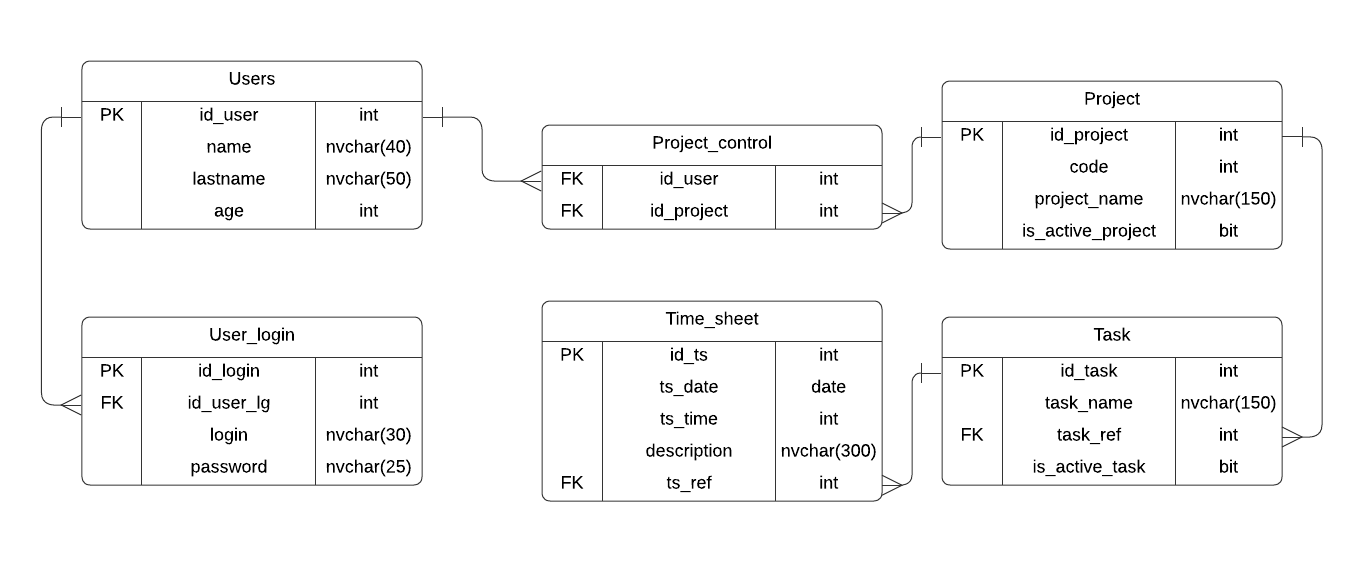
\includegraphics[width=0.9\linewidth]{images/ERFDiagDB}
	\caption{Структура базы данных}
	\label{fig:erfdiagdb}
\end{figure}

Входными данными для портала учета рабочего времени являются:

\begin{itemize}

\item данные о пользователях, включая их имена, фамилии и возраст;
\item учетные данные для авторизации пользователей, такие как логин и пароль;
\item информация о проектах, включая код проекта, название и статус активности;
\item данные о задачах, включая название задачи, ссылку на проект и статус активности;
\item временные данные, включающие дату, время и описание деятельности;
\item контрольные данные, связывающие пользователей с проектами.

Выходными данными являются:

\item отчеты о времени, затраченном на различные проекты и задачи;
\item статистика по активным и завершенным проектам;
\item детализированные записи о выполненных задачах;
\item информация о пользователях, участвующих в различных проектах;
\item данные для авторизации и аутентификации пользователей на портале.
\end{itemize}

\subsubsection{Функциональные требования к программной системе}

В разрабатываемой программно-информационной системе функциональные требования к API предъявляюся со стороны пользовательской части программы.
Должны быть доступны следующие функции программы:

\begin{itemize}
\item Предоставление данных об учетной записи пользователя по логину и паролю.
\item Предоставление данных о проектах, связанных с учетной записью пользователя.
\item Добавление, изменение и редактирование пользовательсих проектов.
\item Предоставление данных о пользовательсих задачах, относящихся к конкретному проекту.
\item Добавление, изменение и редактирование данных о пользовательских задачах.
\item Предоставление данных о проводках, относящихся к конкретной задаче в системе.
\item Добавление, изменение и редактирование данных о проводах.
\item Предоставление данных о проводках за все время и внешними ограничениями с виде промежутка дат.  
\end{itemize}

На рисунке 2.2 в виде диаграммы прецедентов представлены функциональные требования к системее в виде диаграммы прецедентов нотации UML.

\begin{figure}[H]
	\centering
	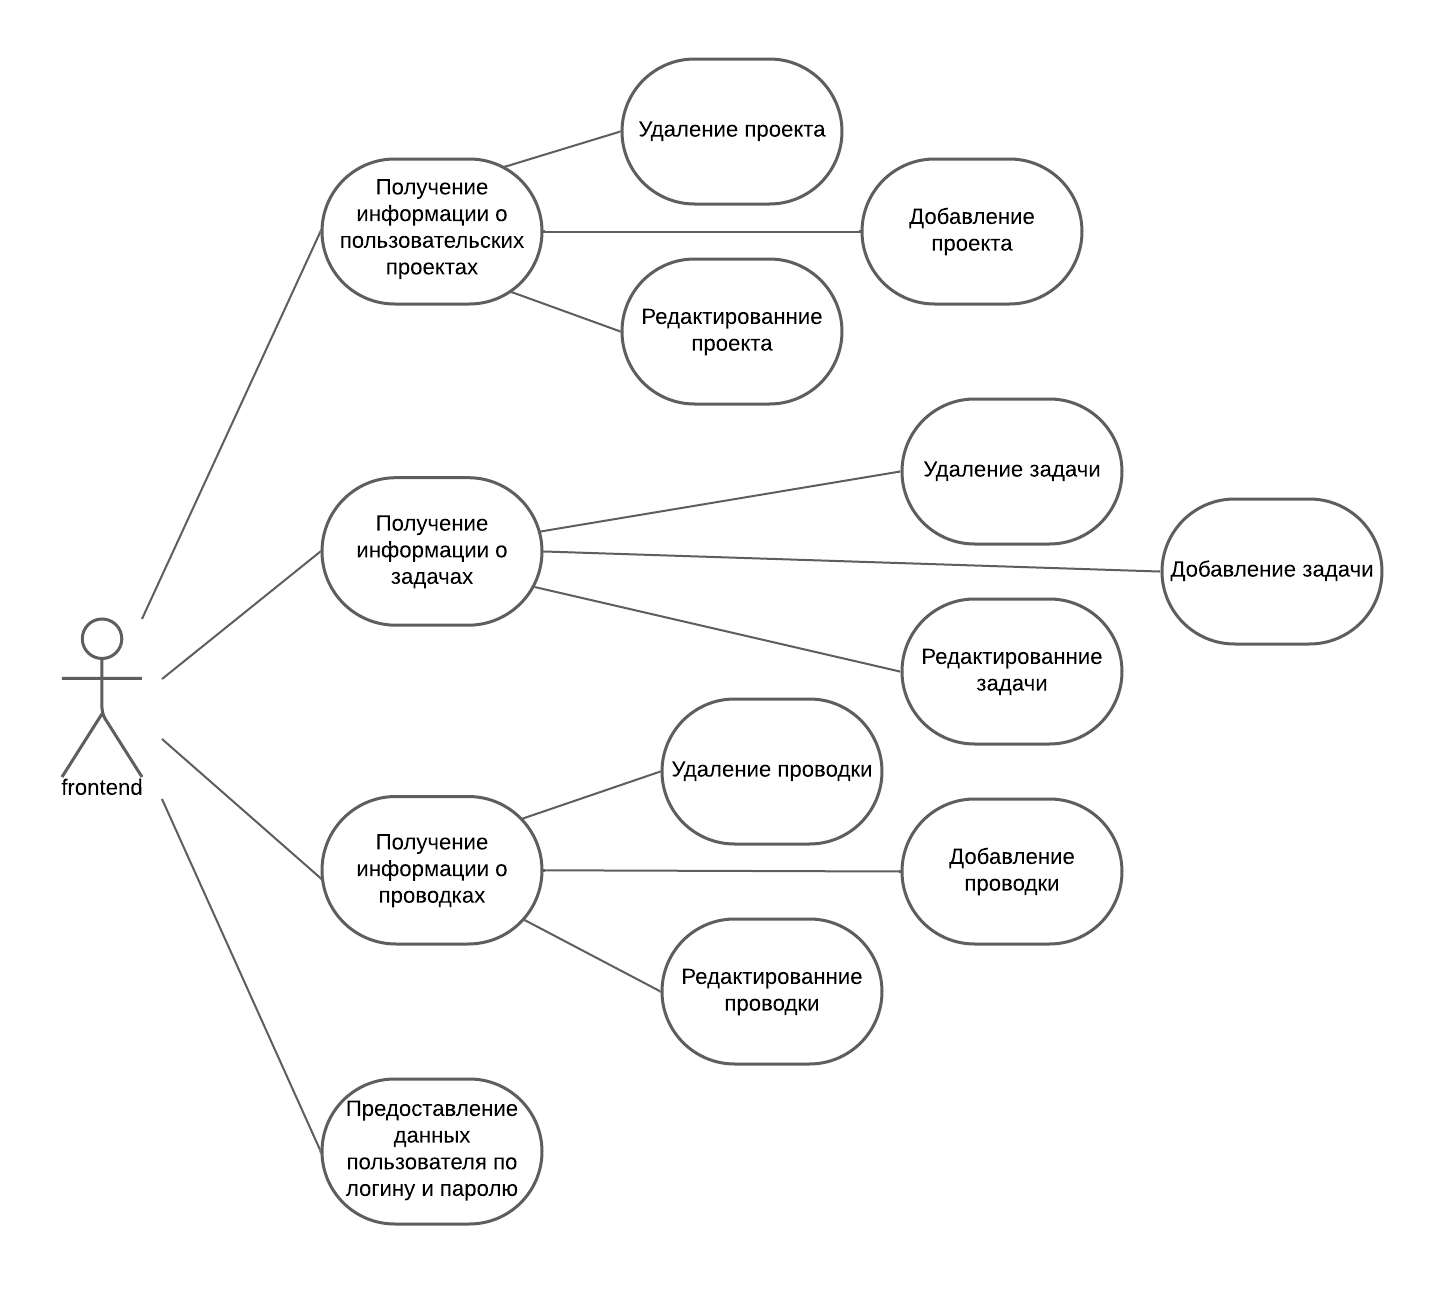
\includegraphics[width=0.9\linewidth]{images/UMLPrecedent}
	\caption{Диаграмма прецедентов}
	\label{fig:umlprecedent}
\end{figure}

\subsubsection{Вариант использования "<Авторизация на веб-портале">}

Заинтересованные лица и их требования: Пользователи веб-портала, которые хотят получить доступ к порталу учета рабочего времени.
Предусловие: Пользователь портала имеет данные для входа от своей учетной записи. Постусловие: Пользователь входит в систему.

Основной успешный сценарий:
\begin{enumerate}
\item Со стороны пользовательской части на сервер отправеляется URI запрос с логином и паролем в формате json файла.
\item Сервер отслеживает запрос и находит пользователя по переданному логину и паролю.
\item Сервер отправляет на frontend json файл с пользовательскими данными.
\end{enumerate}

\subsubsection{Вариант использования "<Получение информации о пользовательских проектах">}

Заинтересованные лица и их требования: Пользователи веб-портала, которые хотят получить доступ к информации о доступных проектах.
Предусловие: Пользователь портала осуществил авторизацию и находится в системе. Постусловие: Пользователь получает данные о проектах.

Основной успешный сценарий:
\begin{enumerate}
	\item Со стороны пользовательской части на сервер отправеляется URI запрос с пользовательским идентификатором в формате json файла.
	\item Сервер отслеживает запрос через контроллер и находит информацию о проектах.
	\item Сервер возвращает на frontend массив всех проектов, доступных данному пользователю.
\end{enumerate}

\subsubsection{Вариант использования "<Добавление нового проекта">}

Заинтересованные лица и их требования: Пользователи веб-портала, которые хотят добаить новый проект под своей учетной записью.
Предусловие: Пользователь портала осуществил авторизацию и находится в системе. Постусловие: Пользователь добавляет новый проект с указанными данными.

Основной успешный сценарий:
\begin{enumerate}
	\item Со стороны пользовательской части на сервер отправеляется URI запрос на добавление проекта с информацией о пользователе.
	\item Сервер отслеживает запрос через контроллер.
	\item Сервер запускает запрос на добавление данных по проекту.
	\item Сервер возвращает на frontend сообщение об успешном добавлении данных по проекту.
\end{enumerate}

\subsubsection{Вариант использования "<Удаление проекта">}

Заинтересованные лица и их требования: Пользователи веб-портала, которые хотят удалить один или несколько доступных проектов.
Предусловие: Пользователь портала осуществил авторизацию и находится в системе. У пользователя есть хотя бы 1 проект. Постусловие: Пользователь удаляет выбранный проект.

Основной успешный сценарий:
\begin{enumerate}
	\item Со стороны пользовательской части на сервер отправеляется URI запрос с кодом проекта, который необходимо удалить в формате json файла.
	\item Сервер отслеживает запрос через контроллер и находит необходимый проект.
	\item Сервер производит каскадное удаление по проекту и всех вложенных данных. 
	\item Сервер возвращает сообщение пользовательской части, об успешном удалении проекта.
\end{enumerate}

\subsubsection{Вариант использования "<Изменение проекта">}

Заинтересованные лица и их требования: Пользователи веб-портала, которые хотят изменить информацию о доступном проекте.
Предусловие: Пользователь портала осуществил авторизацию и находится в системе. У пользователя есть хотя бы 1 проект. Постусловие: Пользователь изменяет выбранный проект.

Основной успешный сценарий:
\begin{enumerate}
	\item Со стороны пользовательской части на сервер отправеляется URI запрос с кодом проекта, который необходимо изменить, а также данные, для изменения выбранного проекта.
	\item Сервер отслеживает запрос через контроллер и находит необходимый проект.
	\item Сервер производит изменение данных по проекту. 
	\item Сервер возвращает сообщение пользовательской части, об успешном изменении проекта.
\end{enumerate}

\subsubsection{Вариант использования "<Получение информации о пользовательских задачах">}

Заинтересованные лица и их требования: Пользователи веб-портала, у которых есть необходимость отслеживать задачи по выбранному проекту.
Предусловие: Пользователь портала осуществил авторизацию и находится в системе. У пользователя есть задачи, относящиеся к конкретному проекту. Постусловие: Пользователь получает данные о задачах по выбранному проекту.

Основной успешный сценарий:
\begin{enumerate}
	\item Со стороны пользовательской части на сервер отправеляется URI запрос с уникальным идентификатором проекта.
	\item Сервер отслеживает запрос через контроллер и находит информацию о задачах.
	\item Сервер возвращает на frontend массив всех задач по выбранному проекту, доступных данному пользователю.
\end{enumerate}

\subsubsection{Вариант использования "<Добавление новой задачи по проекту">}

Заинтересованные лица и их требования: Пользователи веб-портала, которые хотят добаить новую задачу по проекту под своей учетной записью.
Предусловие: Пользователь портала осуществил авторизацию и находится в системе. У пользователя есть хотя бы 1 активный проект. Постусловие: Пользователь добавляет новую задачу по проекту с указанными данными.

Основной успешный сценарий:
\begin{enumerate}
	\item Со стороны пользовательской части на сервер отправеляется URI запрос на добавление задачи с информацией о проекте.
	\item Сервер отслеживает запрос через контроллер.
	\item Сервер запускает запрос на добавление задачи по проекту в соответсвии с переданными данными.
	\item Сервер возвращает на frontend сообщение об успешном добавлении новой задачи.
\end{enumerate}

\subsubsection{Вариант использования "<Удаление задачи по проекту">}

Заинтересованные лица и их требования: Пользователи веб-портала, которые хотят удалить один или несколько доступных задач.
Предусловие: Пользователь портала осуществил авторизацию и находится в системе. У пользователя есть хотя бы одна задача по активному проекту. Постусловие: Пользователь удаляет выбранную задачу.

Основной успешный сценарий:
\begin{enumerate}
	\item Со стороны пользовательской части на сервер отправеляется URI запрос с уникальным идентификатором задачи, которую необходимо удалить.
	\item Сервер отслеживает запрос через контроллер и находит необходимую задачу по проекту.
	\item Сервер производит каскадное удаление по задаче и всех вложенных данных. 
	\item Сервер возвращает сообщение пользовательской части, об успешном удалении задачи.
\end{enumerate}

\subsubsection{Вариант использования "<Редактирование задачи по проекту">}

Заинтересованные лица и их требования: Пользователи веб-портала, которые хотят редактировать информацию о задаче по проекту.
Предусловие: Пользователь портала осуществил авторизацию и находится в системе. У пользователя есть хотя бы одна задача по проекту. Постусловие: Пользователь изменяет выбранную задачу.

Основной успешный сценарий:
\begin{enumerate}
	\item Со стороны пользовательской части на сервер отправеляется URI запрос с уникальным идентификатором задачи, которую необходимо редактировать, а также данные, для изменения выбранной задачи.
	\item Сервер отслеживает запрос через контроллер и находит необходимую задачу.
	\item Сервер производит изменение данных по задаче. 
	\item Сервер возвращает сообщение пользовательской части, об успешном изменении задачи.
\end{enumerate}

\subsubsection{Вариант использования "<Получение данных о проводках по задаче">}

Заинтересованные лица и их требования: Пользователи веб-портала, у которых есть необходимость в просмотра проводок по конкретной задаче.
Предусловие: Пользователь портала осуществил авторизацию и находится в системе. У пользователя есть задачи по проекту и как минимум одна проводка. Постусловие: Пользователь получает данные по проводкам.

Основной успешный сценарий:
\begin{enumerate}
	\item Со стороны пользовательской части на сервер отправеляется URI запрос с уникальным идентификатором задачи, по которой необходимо получить список всех проводок.
	\item Сервер отслеживает запрос через контроллер и находит необходимую задачу.
	\item Сервер запускает скприпт по поиску всех проводок для указанной задачи.
	\item Сервер возвращает список всех проводок по указанной задаче.
\end{enumerate}

\subsubsection{Вариант использования "<Получение данных о проводках за все время">}

Заинтересованные лица и их требования: Пользователи веб-портала, у которых есть необходимость в просмотре проводок за все время.
Предусловие: Пользователь портала осуществил авторизацию и находится в системе. У пользователя есть задачи по проекту и как минимум одна проводка. Постусловие: Пользователь получает данные по проводкам за все время.

Основной успешный сценарий:
\begin{enumerate}
	\item Со стороны пользовательской части на сервер отправеляется URI запрос с уникальным идентификатором задачи, по которой необходимо получить список всех проводок за все время.
	\item Сервер отслеживает запрос через контроллер и находит необходимую задачу.
	\item Сервер запускает скприпт по поиску всех проводок для указанной задачи.
	\item Сервер возвращает список всех проводок за все время.
\end{enumerate}

\subsubsection{Вариант использования "<Добавление новой проводки">}

Заинтересованные лица и их требования: Пользователи веб-портала, у которых есть необходимость в добавлении новой проводки.
Предусловие: Пользователь портала осуществил авторизацию и находится в системе. У пользователя есть задачи по проекту. Постусловие: Пользователь добавляет данные по проводке.

Основной успешный сценарий:
\begin{enumerate}
	\item Со стороны пользовательской части на сервер отправеляется URI запрос с уникальным идентификатором задачи, по которой необходимо добавить проводку.
	\item Сервер отслеживает запрос через контроллер и находит необходимую задачу.
	\item Сервер запускает скприпт на добавление новой проводки, в соотвествии с полученными данными.
	\item Сервер возвращает сообщение на front об успешном добавлении.
\end{enumerate}

\subsubsection{Вариант использования "<Удаление проводки">}

Заинтересованные лица и их требования: Пользователи веб-портала, у которых есть необходимость в удалении проводки.
Предусловие: Пользователь портала осуществил авторизацию и находится в системе. У пользователя есть задачи по проекту и проводки. Постусловие: Пользователь удаляет проводку.

Основной успешный сценарий:
\begin{enumerate}
	\item Со стороны пользовательской части на сервер отправеляется URI запрос с уникальным идентификатором проводки, которую нужно удалить.
	\item Сервер отслеживает запрос через контроллер и находит необходимую проводку.
	\item Сервер запускает скприпт на удаление проводки.
	\item Сервер возвращает сообщение на front об успешном удалении.
\end{enumerate}

\subsubsection{Вариант использования "<Редактирование проводки">}

Заинтересованные лица и их требования: Пользователи веб-портала, у которых есть необходимость в редактировании проводки.
Предусловие: Пользователь портала осуществил авторизацию и находится в системе. У пользователя есть задачи по проекту и проводки. Постусловие: Пользователь редактирует проводку.

Основной успешный сценарий:
\begin{enumerate}
	\item Со стороны пользовательской части на сервер отправеляется URI запрос с уникальным идентификатором проводки, которую нужно редактировать, а так же данные на осонове которых происходит изменение через json файл.
	\item Сервер отслеживает запрос через контроллер и находит необходимую проводку.
	\item Сервер запускает скприпт на редактирование проводки.
	\item Сервер возвращает сообщение на front об изменении проводки.
\end{enumerate}


\subsection{Нефункциональные требования к программной системе}
\subsubsection{Требования к архитектуре}
Серверная часть портала должна быть написана с использованием концепции mvc. База данных должна находится отдельно от файлов проекта для гарантирования целостности данных. Взаимодействие между пользовательской и серверной частью портала должна быть осущестлена по URI запросам с использование протокола HTTPS. Отправка данных должна осуществляться через файлы с расширением .json.

\subsubsection{Требования к безопасности и надежности данных}
Сервер базы данных должен быть написан на языке запросов Microsoft SQL. Сама база данных не должна находится каталогах самого проекта. Подключение к базе данных должно осуществляться через промежуточный файл secret.json, в котором хранится строка подключения к БД. Для обеспечения целостности и предотвращения утечки данных, необходима реализация каскадного удаления, а так же использование транзакций. 

Портал должен выдерживать до 100 запросов в секунду.

\subsubsection{Требования к программному обеспечению}

Для реализации backend части корпоративного портала должны использоваться
следующие технологии:
\begin{itemize}
	\item язык программирования C\#;
	\item библиотека ASP.net MVC.
\end{itemize}

\subsubsection{Требования к аппаратному обеспечению}

Для работы backend части веб-платформы на ASP.NET MVC с использованием Microsoft SQL Server необходим сервер на операционной системе Windows Server. Рекомендуется наличие установленного .NET Framework и SQL Server. Требуется процессор с частотой не менее 2.5 GHz и многопоточностью, дисковое пространство не менее 20 Гб для хранения данных и файлов проекта, а также свободная оперативная память в размере не менее 8 Гб для обеспечения быстрой и стабильной работы приложений. Видеокарта в данном случае не обязательна, так как нагрузка на графический процессор минимальна.

\subsubsection{Требования к оформлению документации}

Разработка программной документации и программного изделия должна производиться согласно ГОСТ 19.102-77 и ГОСТ 34.601-90. Единая система программной документации.

\section{Технический проект}
\subsection{Общая характеристика организации решения задачи}

Необходимо спроектировать и разработать корпоративный портал учета рабочего времени сотрудников. Разрабатываемая программная система предназначена для предоставления комплексного инструмента управления временем, который позволит сотрудникам и менеджерам эффективно отслеживать и управлять временем, затраченным на проекты и задачи.

Основной принцип работы системы заключается в управлении проектами и задачами, а также в учете рабочего времени с помощью таймшитов.

Ключевым компонентом программной системы является база данных для хранения информации о пользователях, проектах, задачах и таймшитах. База данных будет обеспечивать надежное хранение данных и быстрый доступ к ним для выполнения всех операций.

Пользовательский интерфейс будет реализован в виде web-страницы, написанной на языке разметки HTML с применением JS для обработки событий и CSS для описания стилей элементов управления.

Целью разработки данной программной системы является создание эффективного инструмента управления временем в корпоративной среде, который поможет повысить продуктивность сотрудников и оптимизировать процессы проектного управления, способствуя развитию и росту компании.

\subsection{Обоснование выбора технологии проектирования}

Используемые для создания программно-информационной системы языки и технологии отвечают современным практикам разработки, позволяют достичь высокой производительности и отказоустойчивости программы. В частности, связка HTML + CSS позволяет быстро разработать удобные и функциональные пользовательские интерфейсы, а наличие значительного количества фреймворков и библиотек для JS существенно сокращают время, затрачиваемое на разработку функциональной части интерфейса, при этом не причиняя ущерба качеству финального продукта. 

\subsubsection{Описание используемых технологий и языков программирования}

В процессе разработки интерфейса web-сайта использовались следующие языки программирования и программные средства: HTML5, JavaScript, С\# (Razor), CSS.

\subsubsection{Язык разметки HTML5}

HTML5 (HyperText Markup Language, version 5) - это последняя версия стандарта HTML, используемого для создания и структурирования web-страниц и web-приложений. HTML5 представляет собой мощный инструмент для создания современных и интерактивных web-приложений, обеспечивая разработчикам широкий набор возможностей для создания привлекательного и функционального контента в Интернете.

\subsubsection{Языки программирования и фреймворки}

\paragraph{Язык программирования JavaScript}

JavaScript - это высокоуровневый, интерпретируемый язык программирования, который применяется в web-разработке для создания интерактивных элементов на веб-страницах. Он является одним из основных инструментов фронтенд-разработки вместе с HTML и CSS. JS используется для добавления динамического поведения на страницы, обработки событий пользователя, взаимодействия с веб-серверами (через AJAX) и т.д.

\paragraph{Фреймворк Razor для языка программирования C\#}
Razor - это фреймворк, разработанный компанией Microsoft, который используется в ASP.NET для создания динамических web-страниц. Он позволяет разработчикам внедрять код C\# и VB.NET непосредственно в HTML-разметку страницы, что облегчает создание и обслуживание web-приложений. Фреймворк Razor предоставляет мощные средства для работы с данными, логикой и представлениями в веб-приложениях, а также способы для организации кода и повторного использования компонентов интерфейса.

\subsection{Компоненты web-сайта}
Все компоненты web-сайта, реализованного на фреймворке Razor могут принадлежать одной из следующих разновидностей:
\begin{itemize}
\item Частичное представление
\item Представление
\item Классы и шаблоны Razor
\item Разметка Razor
\end{itemize}
Для корректного отображения пользовательского интерфейса, все компоненты любой из этих разновидностей должны лежать в папке Pages или её подпапках. Это гарантирует удобство, простоту и скорость доступа от одного компонента к любому другому компоненту.
Диаграмма компонентов представлена на рисунке ~\ref{fig:comp}

\begin{figure}[H]
	\centering
	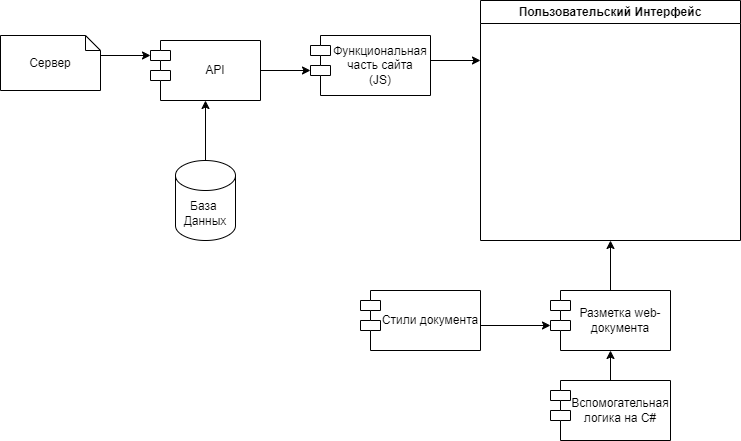
\includegraphics[width=1\linewidth]{images/comp}
	\caption{}
	\label{fig:comp}
\end{figure}

\subsection{Логика клиентской части}
Функциональная часть web-страницы выполнена на языках JavsScript и C\#. Код на JavaScript отвечает за обработку событий и взаимодействие с сервером через API, а код на C\# - за переключение между страницами и компонентами Razor.

\subsubsection{Обработка событий и сообщений от сервера на JS}
Глобально код на JavaScript  можно разделить на две категории: код, выполняющий обработку событий, и код, взаимодействующий с сервером. В более узком плане, код делится по зонам ответственности: класс для работы со страницей авторизации, класс для работы со страницей просмотра и класс для работы со страницей редактирования. Каждая зона ответственности вынесена в отдельный файл; каждый файл внутри логически делится на зоны категорий посредством группирования методов (перечисляются сначала функции для работы с сервером, потом функции для работы с клиентскими событиями, в конце файла идут общие функции, необходимые для построения взаимосвязей между предыдущими группами функций и обработки событий, не предполагающих участия сервера и/или пользователя). Для взаимодействия с сервером (отправка запросов, получение информации) использовалась методология AJAX. Обработка пользовательских событий (ввод информации в текстовые поля, нажатия на кнопки и т.д.) была реализована на "<чистом"> JS (без использования JQuery) с целью экономии ресурсов.
  
\subsubsection{Логика переключения компонентов Razor на С\#}
Логика переключения компонентов Razor реализуется посредством создания контроллера для каждой web-страницы, html-разметка которой расположена в папке "Pages". Контроллер принимает в качестве входных параметров и передаёт на связанную с ним страницу переменные, а также обрабатывает содержимое непосредственно самой web-страницы. Связать URL-адрес страницы и вызов контроллера (т.н. "<назначить странице URL">) можно в основном файле с кодом фреймворка Razor - app.cs через метод "Map()", принимающий на вход URL-адрес, контроллер и необязательные дополнительные параметры.

\subsection{Проектирование пользовательского интерфейса}
На основании требований к пользовательскому интерфейсу, представленных в пункте 2.3.2 технического задания, был разработан графический интерфейс web-сайта. Для создания пользовательского интерфейса используется HTML-разметка с иерархией компонентов Razor Pages.

На рисунке ~\ref{fig:inter3} представлен макет интерфейса формы авторизации. Макет содержит следующие элементы:
\begin{enumerate}
\item Поле ввода логина
\item Поле ввода пароля
\item Кнопка авторизации на портале
\end{enumerate}

\begin{figure}[H]
	\centering
	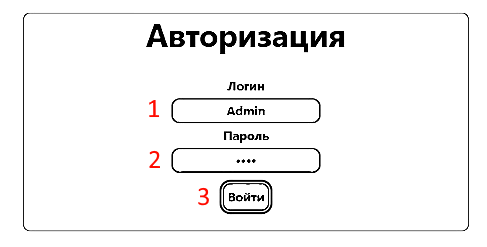
\includegraphics[width=0.5\linewidth]{images/inter3}
	\caption{Макет интерфейса формы авторизации}
	\label{fig:inter3}
\end{figure}

На рисунке ~\ref{fig:inter1} представлен макет интерфейса окна редактирования. Макет содержит следующие элементы:
\begin{enumerate}
	\item Вкладка переключения на окно редактирования
	\item Вкладка переключения на окно просмотра
	\item Кнопка добавления новой записи
	\item Кнопка изменения выбранной записи
	\item Кнопка удаления выбранной записи
	\item Таблица с интерактивными (доступными для выбора по клику правой кнопкой мыши) записями
\end{enumerate}

\begin{figure}[H]
	\centering
	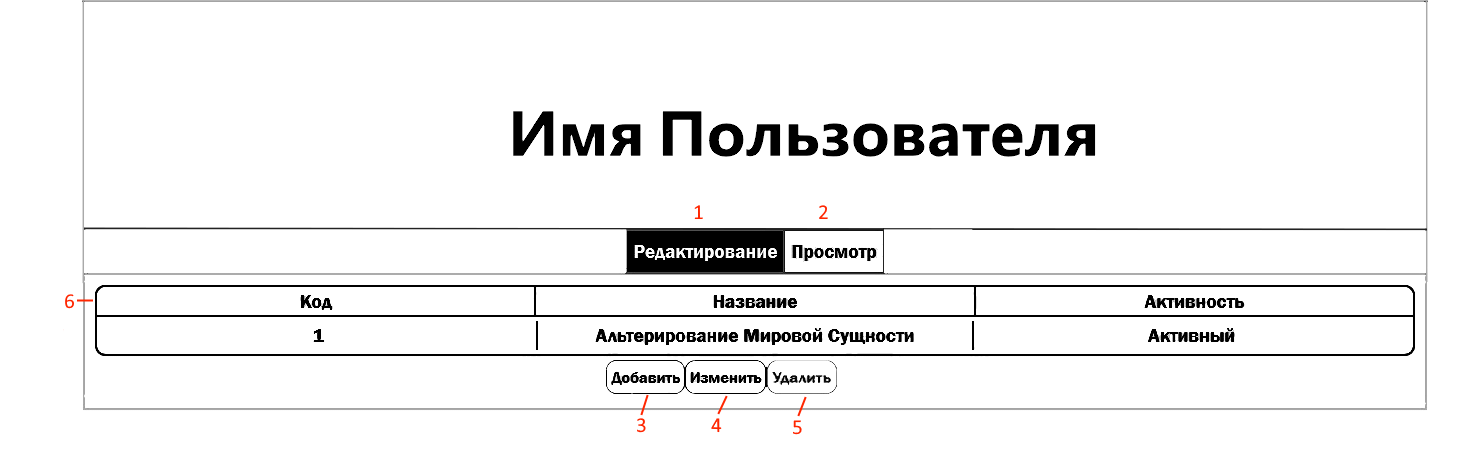
\includegraphics[width=1\linewidth]{images/inter1}
	\caption{Макет интерфейса окна редактирования}
	\label{fig:inter1}
\end{figure}

На рисунке ~\ref{fig:inter2} представлен макет интерфейса окна просмотра. Макет содержит следующие элементы:
\begin{enumerate}
	\item Вкладка переключения на окно редактирования
	\item Вкладка переключения на окно просмотра
	\item Кнопка применения фильтрации по дате
	\item Кнопка сброса фильтрации по дате
	\item Поле ввода даты нижней границы фильтрации
	\item Поле ввода даты верхней границы фильтрации
	\item Таблица с результатами фильтрации или информацией обо всех проводках текущего пользователя
\end{enumerate}

\begin{figure}[H]
	\centering
	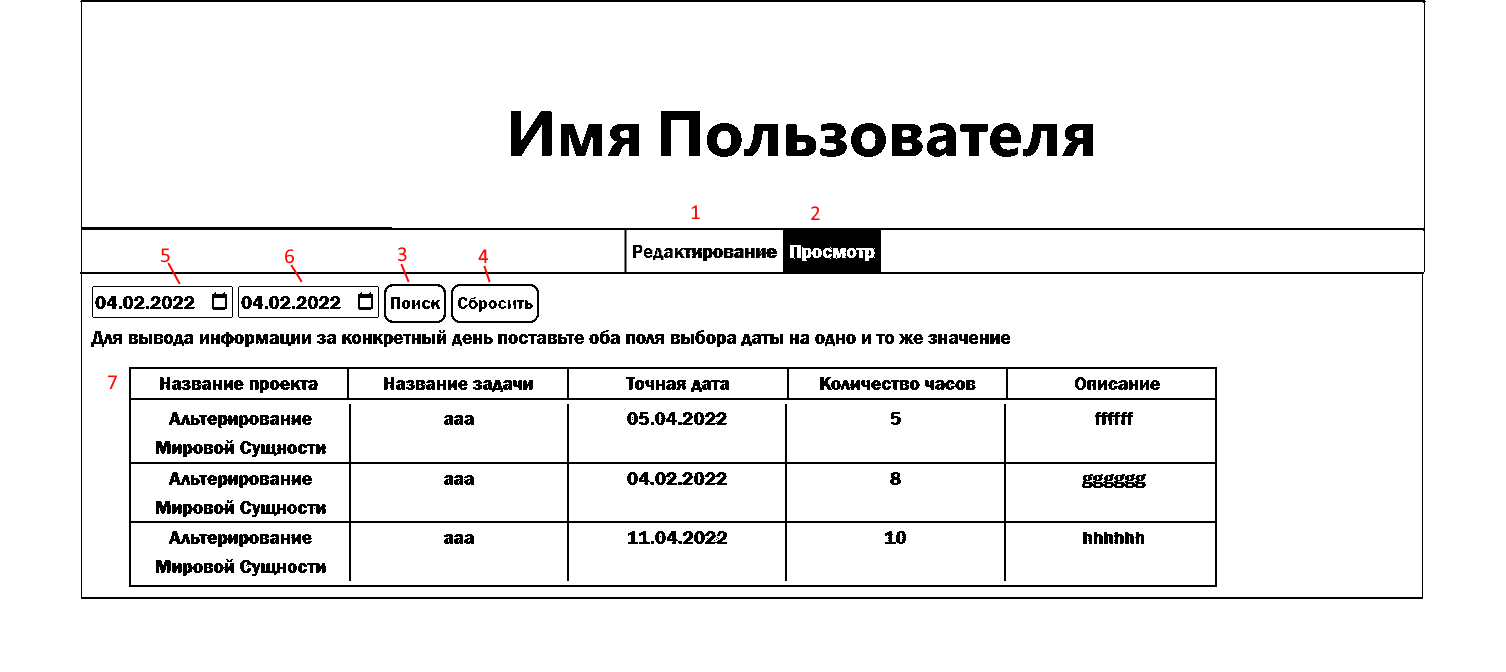
\includegraphics[width=1\linewidth]{images/inter2}
	\caption{Макет интерфейса окна просмотра}
	\label{fig:inter2}
\end{figure}
\ifПрактика{}\else{
   \section{Рабочий проект}
\subsection{Классы, используемые при разработке сайта}

Можно выделить следующий список классов и их методов, использованных при разработке web-приложения (таблица \ref{class:table}). Пример таблицы с уменьшенным межстрочным интервалом.

\renewcommand{\arraystretch}{0.8} % уменьшение расстояний до сетки таблицы
\begin{xltabular}{\textwidth}{|X|p{2.5cm}|>{\setlength{\baselineskip}{0.7\baselineskip}}p{4.85cm}|>{\setlength{\baselineskip}{0.7\baselineskip}}p{4.85cm}|}
\caption{Описание классов Bitrix, используемых в приложении\label{class:table}}\\
\hline \centrow \setlength{\baselineskip}{0.7\baselineskip} Название класса & \centrow \setlength{\baselineskip}{0.7\baselineskip} Модуль, к которому относится класс & \centrow Описание класса & \centrow Методы \\
\hline \centrow 1 & \centrow 2 & \centrow 3 & \centrow 4\\ \hline
\endfirsthead
\caption*{Продолжение таблицы \ref{class:table}}\\
\hline \centrow 1 & \centrow 2 & \centrow 3 & \centrow 4\\ \hline
\finishhead
CMain & Главный модуль & CMain – главный класс страницы web-приложения. После одного из этапов по загрузке страницы в сценарии становится доступным инициализированный системой объект данного класса с именем \$APPLICATION & void ShowTitle(string property\_code = «title», bool strip\_tags = true)
Выводит заголовок страницы
void SetTitle(string title)
Устанавливает заголовок страницы

void ShowCSS(bool external = true, bool XhtmlStyle = true)
Выводит таблицу стилей CSS страницы\\
\hline CFile & Главный модуль & CFile – Класс для работы с файлами и изображениями & array GetFileArray (int file\_id)
Метод возвращает массив, содержащий описание файла (путь к файлу, имя файла, размер) с идентификатором file\_id
\end{xltabular}
\renewcommand{\arraystretch}{1.0} % восстановление сетки

\subsection{Модульное тестирование разработанного web-сайта}

Модульный тест для класса User из модели данных представлен на рисунке \ref{unitUser:image}.

\begin{figure}[ht]
\begin{lstlisting}[language=Python]
from django.test import TestCase
from .models import *
User = get_user_model()


class ShpoTestCases(TestCase):

    def setUp(self) -> None:
        self.user = User.objects.create(username='testtestovich', password='testtestovich', first_name='Sad', last_name='')

    def test_2(self):

        self.assertEqual(self.user.first_name, 'Sad')
        self.assertEqual(self.user.last_name, 'Cat')
        print((self.user))
        print((self.user.first_name))
        print((self.user.last_name))
\end{lstlisting}  
\caption{Модульный тест класса User}
\label{unitUser:image}
\end{figure}

\subsection{Системное тестирование разработанного web-сайта}

На рисунке \ref{main:image} представлена главная страница сайта «Русатом – Аддитивные технологии».
\newpage % при необходимости можно переносить рисунок на новую страницу
\begin{figure}[H] % H - рисунок обязательно здесь, или переносится, оставляя пустоту
\center{\includegraphics[width=1\linewidth]{main1}}
\center{\includegraphics[width=1\linewidth]{main2}}
\center{\includegraphics[width=1\linewidth]{main3}}
\caption{Главная страница сайта «Русатом – Аддитивные технологии»}
\label{main:image}
\end{figure}

На рисунке \ref{menu:image} представлен динамический вывод заголовков, включающий в себя искомые фразы при поиске фраз.

\begin{figure}[ht]
\center{\includegraphics[width=1\linewidth]{menu}}
\caption{Динамический вывод заголовков}
\label{menu:image}
\end{figure}

На рисунке \ref{enter:image} представлен ввод данных для публикации новости.

\begin{figure}[ht]
\center{\includegraphics[width=1\linewidth]{enter}}
\caption{Ввод данных для публикации очень-очень длинной, интересной и полезной новости}
\label{enter:image}
\end{figure}

   \section*{ЗАКЛЮЧЕНИЕ}
\addcontentsline{toc}{section}{ЗАКЛЮЧЕНИЕ}

Преимущества аддитивных технологий заключается в разнообразии процессов, позволяющих применять их в различных областях производства. Существенным ограничением же является и экономическая составляющая, которая не позволит внедрить аддитивное производство повсеместно.
  
Компании, видя, как развиваются информационные технологии, пытаются использовать их выгодно для своего бизнеса, запуская свой сайт для того, чтобы заявить о своем существовании, проинформировать потенциального клиента об услугах или продуктах, которые предоставляет. 
Для продвижения компании «Русатом – Аддитивные технологии» был разработан веб-сайт на основе системы «1С-Битрикс: Управление сайтом».

Основные результаты работы:

\begin{enumerate}
\item Проведен анализ предметной области. Выявлена необходимость использовать 1С-Битрикс.
\item Разработана концептуальная модель web-сайта. Разработана модель данных системы. Определены требования к системе.
\item Осуществлено проектирование web-сайта. Разработана архитектура серверной части. Разработан пользовательский интерфейс web-сайта.
\item Реализован и протестирован web-сайт. Проведено модульное и системное тестирование.
\end{enumerate}

Все требования, объявленные в техническом задании, были полностью реализованы, все задачи, поставленные в начале разработки проекта, были также решены.

Готовый рабочий проект представлен адаптивной версткой сайта. Сайт находится в публичном доступе, поскольку опубликован в сети Интернет.  

}\fi
\addcontentsline{toc}{section}{СПИСОК ИСПОЛЬЗОВАННЫХ ИСТОЧНИКОВ}

\begin{thebibliography}{9}
    \bibitem{aspnetcoreinaction2} Лок, Э. ASP.NET Core в действии, второе издание / Э. Лок. – Москва : Вильямс, 2021. – 800 с. – ISBN 978-1617298301. – Текст: непосредственный.
    \bibitem{proaspnetcoremvc2} Фримен, А. Профессиональное программирование на ASP.NET Core MVC 2 / А. Фримен. – Москва : Эксмо, 2018. – 1018 с. – ISBN 978-1484203989. – Текст: непосредственный.
    \bibitem{proaspnetcore7} Фримен, А. Профессиональное программирование на ASP.NET Core 7 / А. Фримен. – Москва : Вильямс, 2021. – 1080 с. – ISBN 978-1617298974. – Текст: непосредственный.
    \bibitem{aspnetcore5angular} Де Санктис, В. ASP.NET Core 5 и Angular / В. Де Санктис. – Москва : Питер, 2021. – 762 с. – ISBN 978-1800202604. – Текст: непосредственный.
    \bibitem{profcsharpnet2021} Нагель, К. Профессиональное программирование на C\# и .NET, издание 2021 года / К. Нагель. – Москва : Вильямс, 2021. – 1536 с. – ISBN 978-1119797203. – Текст: непосредственный.
    \bibitem{dependencyinjection} Симанн, М. Внедрение зависимостей в .NET / М. Симанн. – Москва : Питер, 2018. – 528 с. – ISBN 978-1617294730. – Текст: непосредственный.
    \bibitem{aspnetcoreidentity} Саркер, С. Профессиональное программирование на ASP.NET Core Identity / С. Саркер. – Москва : Питер, 2021. – 285 с. – ISBN 978-1484259894. – Текст: непосредственный.
    \bibitem{moderncrossplatformdev} Прайс, М. C\# 9 и .NET 5 – Современная кросс-платформенная разработка / М. Прайс. – Москва : Питер, 2021. – 820 с. – ISBN 978-1800568106. – Текст: непосредственный.
    \bibitem{aspnetcoreaction3} Лок, Э. ASP.NET Core в действии, третье издание / Э. Лок. – Москва : Вильямс, 2021. – 900 с. – ISBN 978-1617298288. – Текст: непосредственный.
    \bibitem{professionalaspnetcore} Шустер, М. Профессиональное программирование на ASP.NET Core / М. Шустер. – Москва : ДМК Пресс, 2021. – 600 с. – ISBN 978-1789131823. – Текст: непосредственный.
    \bibitem{proentityframeworkcore} Джонсон, А. Профессиональное программирование на Entity Framework Core / А. Джонсон. – Москва : Вильямс, 2021. – 512 с. – ISBN 978-1787284538. – Текст: непосредственный.
    \bibitem{csharp9dotnet5} Тротт, Дж. C\# 9 и .NET 5 для профессионалов / Дж. Тротт. – Москва : Питер, 2021. – 800 с. – ISBN 978-1484258286. – Текст: непосредственный.
    \bibitem{blazorandaspnetcore} Сантос, Ф. Blazor и ASP.NET Core для профессионалов / Ф. Сантос. – Москва : Вильямс, 2021. – 520 с. – ISBN 978-1801071216. – Текст: непосредственный.
    \bibitem{aspnetcoreanddocker} Вуд, Р. ASP.NET Core и Docker для профессионалов / Р. Вуд. – Москва : Питер, 2021. – 500 с. – ISBN 978-1484260586. – Текст: непосредственный.
    \bibitem{learningcsharp9} Прайс, М. Изучаем C\# 9 и .NET 5 / М. Прайс. – Москва : Питер, 2021. – 500 с. – ISBN 978-1800200723. – Текст: непосредственный.
    \bibitem{aspnetcoreadvanced} Мартин, Р. Продвинутое программирование на ASP.NET Core / Р. Мартин. – Москва : Вильямс, 2021. – 480 с. – ISBN 978-1484261217. – Текст: непосредственный.
    \bibitem{masteringaspnetcore} Смит, Д. Освоение ASP.NET Core / Д. Смит. – Москва : ДМК Пресс, 2021. – 800 с. – ISBN 978-1800200242. – Текст: непосредственный.
    \bibitem{proaspnetcoremvc} Фримен, А. Профессиональное программирование на ASP.NET Core MVC / А. Фримен. – Москва : Вильямс, 2021. – 1040 с. – ISBN 978-1484207208. – Текст: непосредственный.
    \bibitem{beginningaspnetcore} Симпсон, К. Начала программирования на ASP.NET Core / К. Симпсон. – Москва : Питер, 2021. – 620 с. – ISBN 978-1484260890. – Текст: непосредственный.
    \bibitem{aspnetcorewebapi} Уокер, Б. ASP.NET Core Web API / Б. Уокер. – Москва : Вильямс, 2021. – 700 с. – ISBN 978-1801076167. – Текст: непосредственный.
\end{thebibliography}

\ifВКР{\appendix{Представление графического материала}

Графический материал, выполненный на отдельных листах,
изображен на рисунках А.1--А.\arabic{числоПлакатов}.
\setcounter{числоПлакатов}{0}

\renewcommand{\thefigure}{А.\arabic{figure}} % шаблон номера для плакатов

\begin{landscape}

\begin{плакат}
    \includegraphics[width=0.82\linewidth]{плакат1.png}
    \заголовок{Сведения о ВКРБ}
    \label{pl1:image}      
\end{плакат}

\begin{плакат}
    \includegraphics[width=0.82\linewidth]{плакат2.png}
    \заголовок{Цель и задачи разработки}
    \label{pl2:image}      
\end{плакат}

\begin{плакат}
    \includegraphics[width=0.82\linewidth]{плакат3.png}
    \заголовок{Концептуальная модель сайта}
    \label{pl3:image}      
\end{плакат}

\begin{плакат}
    \includegraphics[width=0.82\linewidth]{плакат3.png}
    \заголовок{Еще плакат}
    \label{pl4:image}      
\end{плакат}

\end{landscape}
}\fi
\ifПрактика{}\else{\appendix{Фрагменты исходного кода программы}

main.tex
\lstinputlisting[language=Tex, frame=none]{main.tex}

ТехПроект.tex
\lstinputlisting[language=Tex, frame=none]{ТехПроект.tex}

\ifВКР{
\newpage
\addcontentsline{toc}{section}{На отдельных листах (CD-RW в прикрепленном конверте)}
\begin{center}
\textbf{Место для диска}
\end{center}
}\fi
}\fi
\end{document}
